\section{Introduction}
\label{Introduction}

\subsection{Problem Definition}
Leisure travelling is an impactful industry
whose economic importance significantly improves each
year, contributing to 10.4\% of the global GDP in 2019
~\cite{wttc2018travel}. Despite this, planning for a trip to a
foreign city requires a substantial amount of
time-consuming research. As a result, people often
rely on multiple data sources such as travel
brochures, blogs and vlogs to form a holiday plan and
retrieve the top-rated points of interests (POI) of a site. 
However, a tourist has to compile a timetable
independently even though mediums do not hold the
resources to provide POIs tailored according to the
traveller's preferences and constraints
~\cite{DeChoudhury2010}. 

In literature, offering tourists a personalised route
composed of POIs has been defined as the tourist trip
design problem (TTDP). The TTDP comprises ranking
and selecting POIs that might interest the user and
create a feasible plan. Figure~\ref{TTDP} shows an example
of the TTDP,  where a tourist has to form a timetable
that balances between the POI's rating and location
while satisfying the various trip constraints. 
The TTDP is an NP-hard problem where rigorous
%TODO: ask about rigorous
algorithms only manage to optimise with a small number
of POIs. Therefore, many approximate algorithms,
namely heuristics and meta-heuristic approaches, work
%TODO: ask about this
to converge solutions with complex alternatives to
this problem.Section
~\ref{Literature} provides a detailed review of this problem and its
variants.  


Nevertheless, the few existing systems that provide
users with an itinerary or route require a lengthy
process of manually gathering the users' likes and
constraints or information from past trips. Therefore, we ask the following question: 


\begin{center}

    \textit{Can a system automatically get to know
    what a tourist likes to visit and use this
information to generate a personalised itinerary for a
holiday?}

\end{center}


\begin{figure}[h]
\centering
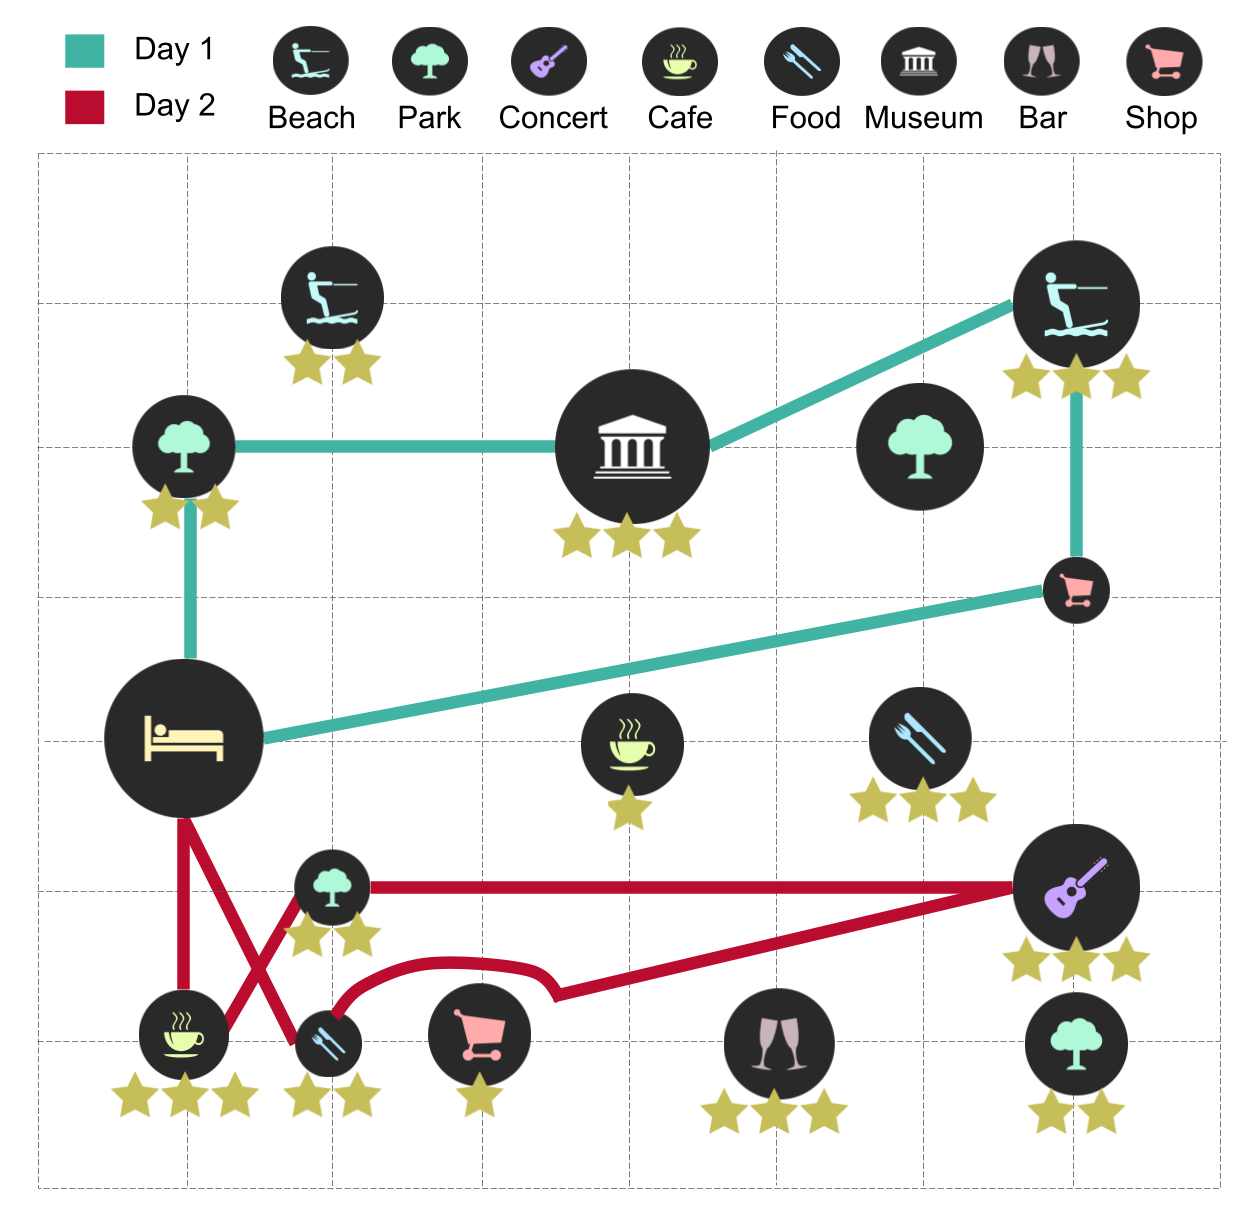
\includegraphics[width=0.65\textwidth]{TTDP.png}
\caption{Example of a tourist planning problem}
\label{TTDP}
\end{figure}

\subsection{Proposed Solution}

To address this problem, we present an application
that helps tourists travel by providing them with a
complete itinerary for their upcoming holiday using
several optimisation algorithms, namely, Genetic
Algorithms (GA) and Particle Swarm Optimisation (PSO).

With the prevalence of social media and data-driven
approaches, we also automate gathering users' POI
desires by scanning their social media profile using
machine learning classification approaches through
Convolutional Neural Networks (CNN).

The results from the evaluation section~\ref{evaluation}
show that we were able to classify the user's photos
and liked pages into a travel interest vector that automatically
describes the user's characteristics. We were also able to provide optimisation
techniques that converge to the timetables with the
best scores given a set of tourist constraints.
In-depth semi-structured interviews with several
participants continued to provide us with further
detail on the accuracy of the user profiling algorithm
and the resulting timetables. 

\subsection{Motivation}

Our primary motivation behind this work is to
introduce the automatic retrieval of user preferences
for other travel planning applications. Currently,
there is no mainstream application that provides
tourists with a fully personalised plan with a quick
and easy to use application.  We were also motivated
by the idea of delivering one centralised system which
organises the whole holiday rather than having to
spend time searching through the excessive amount of
data online. This approach is better than bombarding
potential tourists with many questions to understand
the users' personalities.

\subsection{Why the problem is non-trivial}

Existing algorithms and tourist planners use
heuristics to optimise solutions for the timetable
problem and achievable results in polynomial time
\cite{Vansteenwegen2011}.

Collecting the users' preferences is a
beneficial technique used by businesses to advertise
their products by targeting only a specific audience
\cite{article}.

The problem is non-trivial since we combine both
technologies to provide one system.

\subsection{Aims and Objectives}

This dissertation aims to build an application that
generates a personalised holiday plan according to the
user's travel dates and constraints.


\begin{itemize}
    \item \textbf{Objective 1 (O1)}: Investigate techniques to build travel interest
    profiles automatically from social media interactions.  
    \item \textbf{Objective 2 (O2)}: Explore different optimisation algorithms for
    building personalised travel itineraries using the
    generated travel interest profiles. 
    \item \textbf{Objective 3 (O3)}: Evaluate the
    performance of the personalised travel itinerary
    generator with real users through in-depth
    semi-structured interviews. 

\end{itemize}

We will conduct the interviews by generating a
personalised and non-personalised timetable for a
holiday in Malta to have prior knowledge of the POIs
and compare the effects of both itineraries.

\subsection{Document Structure}

This dissertation is structured as follows; Section~\ref{Literature}
discusses related work relating to existing TTDP
solutions and automatic user preference gathering.
Section~\ref{MethodologyPage} demonstrates the steps taken to create the
whole application along with its underlying mechanism.
Section~\ref{evaluation} will evaluate the performance of the
convolutional neural networks, the optimisation
algorithms and discuss the interview's outcomes.
Finally, section 5 will address the findings obtained
from this research concerning the objectives and some
future improvements.

